\documentclass{article}
\usepackage[utf8]{inputenc}
\usepackage{subfigure}
\usepackage{geometry}
\usepackage{amsmath}
\usepackage{graphicx}
\usepackage{pgfplots}
\usepackage{pgfplotstable}
\usepackage{pgfgantt}
\usepackage{fancyhdr}
\graphicspath{ {./images/} }
\title{Malnourishment and Its Effects on Fruit Fly Survival/Reproduction}
\author{Sirius Chan}
\begin{document}
\maketitle
\thispagestyle{empty}

\newpage

\section{Introduction}

Drosophila melanogaster, are also known as lesser fruit flies. It originates in the African continent and can live for around 50 days, this can be divided into 4 stages\cite{wiki_fly}:

\begin{enumerate}
    \item Embryo (day 0)
    \item Larva (day 1)
    \item Pupa (day 9)
    \item Adult (day 15)
\end{enumerate}

\noindent
They are commonly used in genetic research, especially in the study of inheritance and genetic defects. They are chosen as they have a simple genome of only 4 pairs of chromosomes, and flies with different genetic defects are widely available. This allows research to be carried out on inheritance diseases, such as the study on Alzheimer's disease\cite{alzheimers}.

\noindent\\
It is also used in other medical research and drug developments, being inexpensive to maintain and little care needed to keep them alive, as the only thing they need to survive is food\cite{fly_facts}.

\noindent\\
Other beneficial features include:

\begin{itemize}
    \item They have a short reproduction cycle of 8 - 14 days, so generation/inheritance can be observed in a short period.
    \item Their diet is simple consisting only of carbohydrates and proteins.
    \item They are small at 3mm in length, so many can be kept in a small area.
    \item A female fly produces 30 to 50 eggs in its life span, with a large offspring per generation ratio\cite{fly_facts}.
\end{itemize}

\subsection{Investigation aim}

Last year (2022) the STEM biology class was introduced to culturing fruit flies, I noticed some vials of flies had significantly fewer adult flies after 2 weeks, even though all of them featured the same media mix (fruit fly food) as provided. This left me to wonder how tiny changes in the environment - especially the composition of the media impact the reproduction and survival of fruit flies.

\noindent\\
This investigation aims to figure out how malnourishment affects fruit flies' survival and reproduction through experiments and to answer the question of whether fruit flies will prioritise reproduction when there are not enough nutrients.

\noindent\\
By studying the survival and reproductivity of fruit flies supplied with different amounts of nutrients, a cost-effective formula for the media mix that minimises excess nutrients can be drawn. As well as examine whether lack of nutrients can increase reproductivity rates when starving flies desperately need to give birth to offspring (see hypothesis 1.2.1).

\subsection{Hypotheses}

The hypotheses focus on when the flies do not receive sufficient nutrients, here are two related hypotheses which can be tested in this investigation.

\subsubsection{Hypothesis: When the flies experience malnourishment}

The first hypothesis, when there are not enough nutrients, the fruit flies prioritise reproduction over survival. This could be a result of evolution because, without reproduction, all fruit flies would die out.

\noindent\\
Prioritising reproduction can give the flies an advantage in number when there is not enough resource, giving a greater number of surviving offspring, and avoiding extinction.

\subsubsection{Hypothesis: Carbohydrates and proteins have different functions}

Carbohydrates, such as glucose provide most of the energy for the flies' survival through respiration. The hypothesis believes that carbohydrates and proteins are responsible for specific and irreplaceable functions, rather than being able to replace each other when there is a deficiency.

\noindent\\
Therefore, when there is an insufficient amount of carbohydrates, many adult flies die as they cannot carry out their normal respiration. When there are not enough proteins, the flies should still be able to survive with the energy from carbohydrates but will experience stunted growth and reproduction. Protein is mainly responsible for the growth of organisms.

\subsection{Objectives}

The main objective of this investigation is to evaluate the data collected through experiments, to support or disprove the hypotheses.

\noindent\\
To answer the hypothesis, I will need to:

\begin{enumerate}
    \item Produce a good number of vials containing media mix, in each vial the composition of the media mix is slightly different.
    \item Put the flies into the vials and culture them.
    \item Regularly record data on the reproduction and number of surviving flies.
\end{enumerate}

\noindent\\
To support the hypothesis on malnourishment:

\begin{itemize}
    \item Both the reproduction rate and survival rate are "high" when there are sufficient nutrients.
    \item "Insufficient" nutrients a significant drop in survival rate, while the reproduction rate remains relatively high.
    \item Many larvae will not grow up into adults when they don't have sufficient nutrients as a result of low survival rates.
\end{itemize}

\noindent\\
To support the hypothesis on the different functions of carbohydrates and proteins:

\begin{itemize}
    \item A Decrease in the concentration of carbohydrates only leads to fewer surviving adult flies.
    \item A Decrease in the concentration of proteins only leads to less reproduction.
\end{itemize}

\noindent
(I'm only writing this because of the criteria form.) Since the investigation aims to identify how changes in the culture media affect the behaviour of flies, the best approach would be to create fruit fly cultures with different compositions for the media.

\section{Investigation plan}

The investigation will be divided into 3 stages:

\begin{enumerate}
    \item Preparation: Where the vials are set up and ready to start the experiment.
    \item Recording: Start the experiment, and record all relevant information.
    \item Evaluation: Evaluate the hypotheses using the data recorded, and conclude.
\end{enumerate}

\begin{center}
    \begin{ganttchart}[y unit title=0.4cm,
    y unit chart=0.5cm,
    vgrid,hgrid, 
    title label anchor/.style={below=-1.6ex},
    title left shift=.05,
    title right shift=-.05,
    title height=1,
    progress label text={},
    bar height=0.7,
    group right shift=0,
    group top shift=.6,
    group height=.3]{1}{24}
    %labels
    \gantttitle{2023}{24} \\
    \gantttitle{March}{3} 
    \gantttitle{April}{8} 
    \gantttitle{May}{8} 
    \gantttitle{June}{5} \\
    %tasks
    \ganttbar{Make media mix}{1}{1} \\
    \ganttbar{Sort by gender}{12}{12} \\
    \ganttbar{Putting into vials}{13}{13} \\
    \ganttbar{Record data}{14}{23} \\
    \ganttbar[progress=0]{Evaluations}{24}{24}
    % %relations 
    \ganttlink{elem0}{elem1} 
    \ganttlink{elem1}{elem2} 
    \ganttlink{elem3}{elem4} 
    \end{ganttchart}
\noindent
(Diagram not to scale)
\end{center}


\noindent
There is a month-long gap between making the media mix and sorting the flies by gender, this is because the ordered flies do not arrive until May.

\subsection{Preparing vials}

A prepared vial should contain:

\begin{itemize}
    \item The media mix.
    \item A set amount of male flies.
    \item A set amount of female flies.
\end{itemize}

\noindent
The school has ordered some flies which will arrive after the Easter holidays, so before that, the only thing that can be prepared is the media mix in the vials. It can be prepared early and then refrigerated until the experiment starts.

\subsubsection{Media mix formula}

I asked for the formula of the media mix Dr Bass used last year, as it was working just fine. Here is the formula I was given.

{
\centering
\begin{tabular}{|c|c|}
  \hline
  Item & Amount\\
  \hline
  \hline
  Distilled water & 500ml\\
  Agar & 5g\\
  Brewers yeast & 50g\\
  Sucrose & 50g\\
  Propionic acid & 2ml\\
  Methyl 4-hydroxybenzoate & 0.5g\\
  Ethanol & 1.3ml\\
  \hline
\end{tabular}
\par
}

\noindent\\
This formula is simple, with the sucrose providing the carbohydrates for the flies, and the brewers yeast providing the proteins.

\noindent\\
I've also tried looking up different recipes for the media mix, the one that is most similar to the recipe I was given\cite{sim_recipe} also uses yeast as the source of protein. But instead of sucrose, it uses soy flour, cornmeal and molasses as sources of carbohydrates.

\noindent\\
Many recipes I've found online also suffer from the same issues, they seemed to be optimised with multiple ingredients making up the carbohydrates portion of the media mix. In contrast, Dr. Bass' recipe only uses sucrose for all carbohydrate needs of the flies, so it would be easier to make a media mix.

\noindent\\
All media mix recipes seemed to have a few things in common:

\begin{itemize}
    \item Yeast for protein.
    \item Syrup, flour or other plant extracts for carbohydrates.
    \item Propionic acid or nipagin as preservatives.
    \item Antibiotics such as phosphoric-propionic acid, if needed\cite{diet}.
    \item Finally, agar to solidify everything into a gel-like substance.
\end{itemize}

\noindent
After considering the complexity of different recipes for media mixes, I've decided to go with Dr. Bass' recipe where each part of the media only consists of one ingredient.


\subsection{Investigation approach}

By culturing fruit flies using media mixed with different concentrations of sucrose and yeast, the number of flies alive and larvae in these different vials can show how changing the number of nutrients they receive impacts their survival and reproduction.

\subsubsection{Variables}

The independent variable will be the composition of the vials. Each vial will be made of slightly different concentrations of sucrose and yeast, starting from the 75 (sucrose) and 75 (yeast) $g/dm^3$ which is the same as Dr Bass' formula.

\noindent\\
Below are the sucrose and yeast concentrations of the different vials.\\

{
\centering
\begin{tabular}{|c|c|c|}
  \hline
  Vial & Sucrose ($g/dm^3$) & Yeast ($g/dm^3$)\\
  \hline
  \hline
  1 & 75 & 75\\
  2 & 67.5 & 67.5\\
  3 & 60 & 60\\
  4 & 52.5 & 52.5\\
  5 & 45 & 45\\
  6 & 37.5 & 37.5\\
  7 & 30 & 30\\
  8 & 22.5 & 22.5\\
  9 & 15 & 15\\
  10 & 0 & 0\\
  \hline
\end{tabular}
\begin{tabular}{|c|c|c|}
  \hline
  Vial & Sucrose ($g/dm^3$) & Yeast ($g/dm^3$)\\
  \hline
  \hline
  11 & 60 & 75\\
  12 & 45 & 75\\
  13 & 30 & 75\\
  14 & 15 & 75\\
  15 & 0 & 75\\
  \hline
  16 & 75 & 60\\
  17 & 75 & 45\\
  18 & 75 & 30\\
  19 & 75 & 15\\
  20 & 75 & 0\\
  \hline
\end{tabular}
\par
}
\noindent\\
(Vials 1 - 10 for hypothesis on malnourishment, 11 - 20 for protein/carbohydrates roles hypothesis.)

\noindent\\
The dependent variables are the things being measured, in this experiment there are multiple things to be measured.

\begin{itemize}
    \item Number of active (alive) fruit flies.
    \item Number of inactive (dead) fruit flies.
    \item Number of larvae.
    \item Number of pupa.
\end{itemize}

\noindent
Decreasing the concentrations of sucrose and yeast effectively reduces the amount of nutrients the flies can take in, as each fly can only consume so much media. The rest of the variables will be kept the same across all vials by placing all the vials in around the same location.

\subsubsection{Data collection}

The number of flies alive, larvae, and pupa can be counted, and the number can be recorded in a note-taking app.

\noindent\\
From experience, the number of pupae can be counted easily, as they tend to stay on the side of the vials during pupariation. However, the number of active flies in a vial can be difficult to count, as they move around a lot. A way to give a good estimate of the actual number of flies is to just try to count all of them quickly, so they don't have as much time to move around.

\noindent\\
The number of larvae in a vial can be even more difficult to estimate, as they usually stay inside the opaque food medium until they reach the pupal stage\cite{in_medium}. So only larvae very close to the edge of the vial are visible and can be counted.

\subsection{Methodology}

The experiment uses \emph{drosophilas}, as it is low cost and works well, and being the only species I have slight experience culturing.

\noindent\\
Male and female drosophilas can also be differentiated with the naked eye, making the process of putting an equal amount of files of each gender simpler and quicker.\\

\begin{center}
\includegraphics[width=5cm]{fm-flies}
\noindent\\
(Smaller, back-ended ones are male. Larger, striped ones are females.)
\end{center}

\subsubsection{Preparing media mix (23 - 24th March)}

Materials needed for the 20 vials of media are:\\

{
\centering
\begin{tabular}{|c|c|}
  \hline
  Item & Amount\\
  \hline
  \hline
  Distilled water & 300ml\\
  Agar & 3g\\
  Propionic acid & 1.2ml\\
  Methyl 4-hydroxybenzoate & 0.3g\\
  Ethanol & 1.3ml\\
  Brewers yeast & 15g\\
  Sucrose & 15g\\
  30ml vials & 20x\\
  \hline
\end{tabular}
\par
}

\noindent\\
3 different solutions are made in bulk before mixing them into the individual vials:

\begin{enumerate}
    \item Weigh out agar and place it in a 1-litre Simax reagent bottle (a large glass container).
    \item Add 200 ml of distilled water, propionic acid and methyl 4-hydroxybenzoate (dissolved in 3 ml of ethanol) to the bottle.
    \item In a smaller bottle, dissolve 15g of brewer's yeast (powder) in 50ml of distilled water.
    \item In another bottle, dissolve 15g of sucrose in 50ml of distilled water.
    \item Leave the 3 bottles cap loose and autoclave (sterilise by heating).
    \item Place all the bottles in a 55\textcelsius\space water bath to allow equilibriation.
\end{enumerate}

\newpage
\noindent
This prepares:

\begin{itemize}
    \item 50ml of 300g/dm$^3$ sucrose solution.
    \item 50ml of 300g/dm$^3$ brewer's yeast solution.
    \item 200ml solution containing agar, methyl 4-hydroxybenzoate (dissolved in ethanol), and propionic acid.
\end{itemize}

\noindent
Referencing the table on page 6, prepare the 20 vials:

\begin{enumerate}
    \setcounter{enumi}{6}
    \item Add 10ml of the agar solution to each vial.
    \item Mark each vial with a number 1 - 20, and the sucrose and yeast concentration it should have.
    \item Add appropriate amounts of sucrose and yeast solution into each vial. (e.g. 75dm$^3$ can be made by adding 5ml of that solution, while 37.5dm$^3$ can be made by adding only 2.5ml of that solution.)
    \item Add extra distilled water to pad volume to 20ml for all vials, it also dilutes media to the desired concentration.
    \item Cap vials for them to set in a fridge.
\end{enumerate}

\begin{figure}[ht]
  \centering
  \subfigure[All the empty vials]{\includegraphics[width=0.45\textwidth]{vials-before}}
  \hfill
  \subfigure[Vials filled with the correct media mixes]{\includegraphics[width=0.45\textwidth]{vials-after}}
\end{figure}

\subsubsection{Starting the culture (3 - 4th May)}

Each vial should have the same number of male and female flies, to determine \emph{how many} flies of each sex to put in the vials, a rough estimate is used to find the male-to-female flies ratio in the large stock vial. The estimation is done by counting the number of each gender of flies from multiple images - taken using a mobile phone.

\noindent\\
After the estimation, it was decided each vial should have 4 males and 5 females, as the two genders exist in the stock vial in ratios of 4:5.

\newpage
\noindent
Here are the steps I used to do that:

\begin{enumerate}
    \item Use a fly anesthetiser, such as FlyNap on the stock vial to put the flies unconscious.
    \item Prepare some iced water and a petri dish placed in the water. This is used to keep the flies asleep after they are poured out of the anaesthetic-filled container. (The coldness keeps ectothermic animals like flies asleep)
    \item Pour the unconscious flies onto the petri dish.
    \item Use a watercolour brush to pick up the correct amount of flies into each vial. (Yes, the files can be picked up with the brush)
\end{enumerate}

\noindent
Instead of using the plastic cap of the vials, tape and cotton can be used to keep the flies inside without sealing off fresh air, which is needed for respiration.

\noindent\\
Since the flies are being put into the vials across a span of 2 days, I refrigerate the vials immediately after the flies are put in, and only take them out after the last vial is ready. This is to prevent some vials from getting an early head start.

\begin{center}
\includegraphics[width=5cm]{to-vials}
\noindent\\
(Image showing the larger blue stock vial of flies and 20 smaller vial cultures)
\end{center}

\noindent
On 5th May, after all vials of cultures were refrigerated for at least a night (for fairness) they were taken out for the experiment to start.

\subsubsection{Recording data (12th May - 19th June)}

Data is recorded every week, the first recording is on day 7 (12th May) and the last recording in day 45 (19th June).

\noindent\\
A mobile note-taking app is used to take down the numbers of active flies for each vial, each week.

\noindent\\
The number of flies in the larva and pupa stages of life will also need to be included in one of the recordings, as it is needed to calculate the rates of reproduction, survival, and reproduction-survival ratio in support of or invalidating the two hypotheses.

\begin{itemize}
    \item \emph{Number of active flies} is difficult to count accurately without FlyNap, as they move around a lot and wake up from sleep very quickly. But by counting all flies quickly, it can be closer to the true value.
    \item \emph{Number of larvae} can only be estimated, as they dig into the opaque culture media - only ones near the wall of vials can be seen and counted.
    \item \emph{Number of pupae} can be accurately counted, as they make clear distinct shapes on the walls and do not move.
\end{itemize}

\subsubsection{Evaluation: malnourishment hypothesis}

The hypothesis claims that fruit flies should prioritise reproduction over survival when malnourished - which should first be defined.

\noindent\\
When there are sufficient nutrients, the main limiting factors for the number of flies after a set period, are availability of space and speed of reproduction, rather than the concentration of nutrients. Therefore, changing the concentration of nutrients will have little effect on the number of flies. However, when there are insufficient nutrients in the media, any changes to this limiting factor will have large effects on this number of flies.

\noindent\\
To identify the concentration where flies are malnourished, plot a graph of the number of flies alive after 30 days against the concentration. An inflex point should separate the steeper slope to the left, and the gentler slope to the right.

\noindent\\
To show support for the hypothesis, the experiment must show reproduction decreasing at a slower rate than survival as the concentration of nutrients in media decreases.

\begin{align*}
  \text{reproduction rate}&=\frac{\text{no. of larvae + pupa}}{\text{initial no. of flies}}\\
  \text{survival rate}&=\frac{\text{no. of adult flies}}{\text{no. of larvae + pupa}}\\
  \text{reproduction-survival ratio}&=\frac{\text{reproduction rate}}{\text{survival rate}}
\end{align*}

\noindent
The reproduction rate measures how many offspring can each fly give, and the survival rate measures the likeliness of an offspring surviving into adulthood. These rates should be independent of the initial number of flies, so that experiment results can be reproduced and compared.

\subsubsection{Evaluation: carbohydrate/protein specific functions}

The hypothesis claims that carbohydrates and protein have specific and irreplaceable functions from each other - decreasing concentrations of carbohydrates mostly negatively impacts survival rate and protein for reproductivity.

\noindent\\
To support the hypothesis, the experiment must show decreasing carbohydrate concentration leads to an increase in the reproduction-survival ratio, but decreasing protein decreases the ratio.

\subsection{Limitations}

\begin{itemize}
    \item The experiment uses cultures with sucrose/yeast concentrations of 0 to 75 g/dm$^3$ in intervals of 7.5g/dm$^3$, this interval may not be dense enough for a representative result.
    \item The subinterval where nutrients are insufficient may not be well covered. For example, if nutrients are insufficient below 30g/dm$^3$, there will only be 4 vials covering this interval, results may be prone to random error.
    \item Every fly is unique and can differ in terms of reproductivity and survival, even if exposed to the same environment, this also contributes to random error.
\end{itemize}

\section{Evalutaion}

\subsection{Recordings}

The day which the cultures started (day 0) is 7th May.\\

{
\centering
\begin{tabular}{|c|c|c|c|c|c|c|c|c|}
  \hline
  Vial & Sucrose & Yeast & Day 7 & Day 14 & Day 31 & Day 38 & Day 45 & Pupa + larvae\\
  \hline
  \hline
  1 & 75 & 75 & 8 & 8 & 44 & 128 & 44 & 73\\
  2 & 67.5 & 67.5 & 8 & 6 & 51 & 94 & 14 & 69\\
  3 & 60 & 60 & 8 & 7 & 44 & 69 & 2 & 73\\
  4 & 52.5 & 52.5 & 9 & 7 & 47 & 74 & 3 & 86\\
  5 & 45 & 45 & 7 & 9 & 43 & 83 & 2 & 82\\
  6 & 37.5 & 37.5 & 9 & 6 & 36 & 65 & 3 & 51\\
  7 & 30 & 30 & 7 & 10 & 40 & 54 & 39 & 39\\
  8 & 22.5 & 22.5 & 9 & 8 & 38 & 54 & 26 & 30\\
  9 & 15 & 15 & 6 & 8 & 5 & 21 & 12 & 3\\
  10 & 0 & 0 & 2 & 0 & 0 & 0 & 0 & 0\\
  \hline
  11 & 60 & 75 & 7 & 7 & 47 & 61 & 75 & 69\\
  12 & 45 & 75 & 8 & 7 & 16 & 57 & 80 & 45\\
  13 & 30 & 75 & 7 & 7 & 28 & 37 & 74 & 80\\
  14 & 15 & 75 & 9 & 6 & 11 & 20 & 3 & 87\\
  15 & 0 & 75 & 6 & 0 & 13 & 0 & 0 & 108\\
  \hline
  16 & 75 & 60 & 6 & 9 & 66 & 89 & 4 & 35\\
  17 & 75 & 45 & 9 & 6 & 46 & 63 & 68 & 38\\
  18 & 75 & 30 & 8 & 6 & 42 & 80 & 1 & 64\\
  19 & 75 & 15 & 8 & 8 & 5 & 4 & 0 & 11\\
  20 & 75 & 0 & 7 & 7 & 0 & 0 & 0 & 0\\
  \hline
\end{tabular}
\par
}

\begin{itemize}
    \item Day n shows the number of flies alive on the day of recording.
    \item The number of pupa and larvae is recorded on day 14 in the second recording when they first appeared. As they become an unidentifiable blur in later recordings.
\end{itemize}

\subsection{Finding interval of insufficient nutrients}

The hypothesis on malnourishment can be supported if experiment data shows the reproduction-to-survival ratio increases as nutrients become more scarce. However, the ratio may behave differently when nutrients become abundant. For example, a trend that occurs when there are insufficient nutrients may not continue into the interval where nutrients are sufficient.

\noindent\\
Referencing 2.3.4, the steeper interval where nutrients are the main limiting factor, and the gentler interval where it is not, are separated by an inflex point of changing slope. This change in trend can be identified by plotting the number of flies alive against the concentration of media mix.

\noindent\\
Only vials numbered 1 - 10 are included in the graph, as both the concentration of sucrose and protein decreases proportionally so that we can identify the interval where there is a general insufficiency of \emph{nutrients}, rather than just insufficiency of sucrose or protein.

\begin{center}
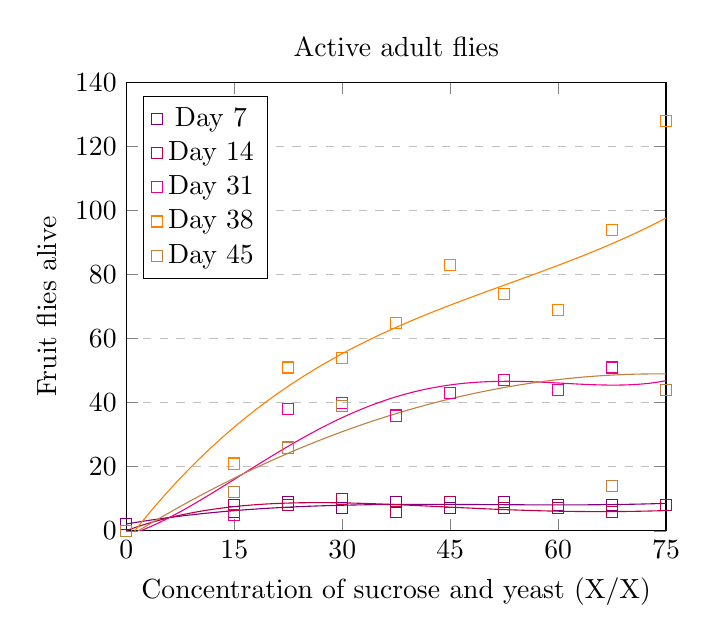
\begin{tikzpicture}
  \begin{axis}[
    title={Active adult flies},
    xlabel={Concentration of sucrose and yeast (X/X)},
    ylabel={Fruit flies alive},
    xmin=0, xmax=75,
    ymin=0, ymax=140,
    xtick={0,15,30,45,60,75},
    ytick={0,20,40,60,80,100,120, 140},
    legend pos=north west,
    ymajorgrids=true,
    grid style=dashed,
]

  \addplot[
    only marks,
    color=violet,
    mark=square,
  ]
  coordinates{
    (0,2)(15,6)(22.5,9)(30,7)(37.5,9)(45,7)(52.5,9)(60,8)(67.5,8)(75,8)
  };
  \addlegendentry{Day 7}
    
  \addplot[
    only marks,
    color=purple,
    mark=square,
  ]
  coordinates {
    (0,0)(15,8)(22.5,8)(30,10)(37.5,6)(45,9)(52.5,7)(60,7)(67.5,6)(75,8)
  };
  \addlegendentry{Day 14}
  

  \addplot[
    only marks,
    color=magenta,
    mark=square,
  ]
  coordinates {
    (0,0)(15,5)(22.5,38)(30,40)(37.5,36)(45,43)(52.5,47)(60,44)(67.5,51)(75,44)
  };
  \addlegendentry{Day 31}

  \addplot[
    only marks,
    color=orange,
    mark=square,
  ]
  coordinates {
    (0,0)(15,21)(22.5,51)(30,54)(37.5,65)(45,83)(52.5,74)(60,69)(67.5,94)(75,128)
  };
  \addlegendentry{Day 38}

  \addplot[
    only marks,
    color=brown,
    mark=square,
  ]
  coordinates {
    (0,0)(15,12)(22.5,26)(30,39)(67.5,14)(75,44)
  };
  \addlegendentry{Day 45}

  \addplot [
    domain=0:75, 
    samples=100, 
    color=violet,
    ]
    {0.000051*x^3-0.00778*x^2+0.382514*x+2.136369};
  \addplot [
    domain=0:75, 
    samples=100, 
    color=purple,
    ]
    {-0.000001*x^4+0.000278*x^3-0.024972*x^2+0.814395*x+0.075425};
  \addplot [
    domain=0:75, 
    samples=100, 
    color=magenta,
    ]
    {0.0000084*x^4-0.001285*x^3+0.048214*x^2+0.714434*x-1.578422};
  \addplot [
    domain=0:75, 
    samples=100, 
    color=orange,
    ]
    {0.00025*x^3-0.039775*x^2+2.923647*x-3.334842};
  \addplot [
    domain=0:75, 
    samples=100, 
    color=brown,
    ]
    {-0.009425*x^2+1.39034*x-2.272553};
  \end{axis}
\end{tikzpicture}
\end{center}

\noindent
The graph shows that the number of flies remained largely unchanged in the first 2 recordings, as flies in larvae and pupa stages were not spotted until the second recording. As a result, the number of flies in the first 2 recordings has little study value, except for vial 10 with no sucrose or yeast at all, which confirmed that flies cannot survive without nutrients as no flies were alive after 2 weeks.

\noindent\\
There is a clear inflexion point on day 31. To the left of 45g/dm$^3$, the number of flies is directly proportional to the concentration of sucrose and yeast and flat to the right. This tells us that the concentration of media mix is the main limiting factor before 45g/dm$^3$, and the interval of insufficient nutrients is between 0 to 45g/dm$^3$.

\noindent\\
On day 38 there is only a vague inflection point at 30g/dm$^3$, this is different from what's observed on day 31. Concentration is still a limiting factor when media concentration is high, although with fewer effects. One possibility is that the culture media has already begun to run out, and vials with lower concentrations would run out earlier as the media would be used at a higher rate, leaving flies in cultures of lower concentration without food for longer, reducing the number of flies that survived.

\noindent\\
On day 45 there are significantly fewer flies compared to the previous recording, this is mainly because of the culture media starting to run out for all vials. So the numbers in day 45 should be treated as abnormal and ignored.

\subsection{Evalutating hypothesis: flies will prioritise reproduction}

The hypothesis believes that the reproduction rate will decrease slower than the survival rate as nutrients become more and more insufficient. In other words, the reproduction-survival ratio should increase as the concentration of media decreases, and the line of best fit would have a negative slope.

\noindent\\
Only adult fly numbers from days 31 and 38 can be used as other recordings are not good representations of the culture.

$$\text{reproduction-survival ratio}=\frac{\text{reproduction rate}}{\text{survival rate}}$$

% \begin{table}[h]
% \centering
% \begin{tabular}{|c|c|c|c|}
%   \hline
%   Concentration & larvae + pupa & Ratio (day 31) & Ratio (day 38)\\
%   \hline
%   \hline
%   0 & 0 & 0 & 0\\
%   15 & 3 & 0.2 & 0.0476\\
%   22.5 & 30 & 2.6316 & 1.9608\\
%   30 & 39 & 4.225 & 3.1296\\
%   37.5 & 51 & 8.0278 & 4.4462\\
%   45 & 82 & 17.3747 & 9.0013\\
%   52.5 & 96 & 21.7872 & 13.8378\\
%   60 & 73 & 13.4571 & 8.5813\\
%   67.5 & 69 & 10.3725 & 5.6277\\
%   75 & 75 & 14.2045 & 4.8828\\
%   \hline
% \end{tabular}
% \end{table}

\begin{center}
  \begin{minipage}{.45\linewidth}
  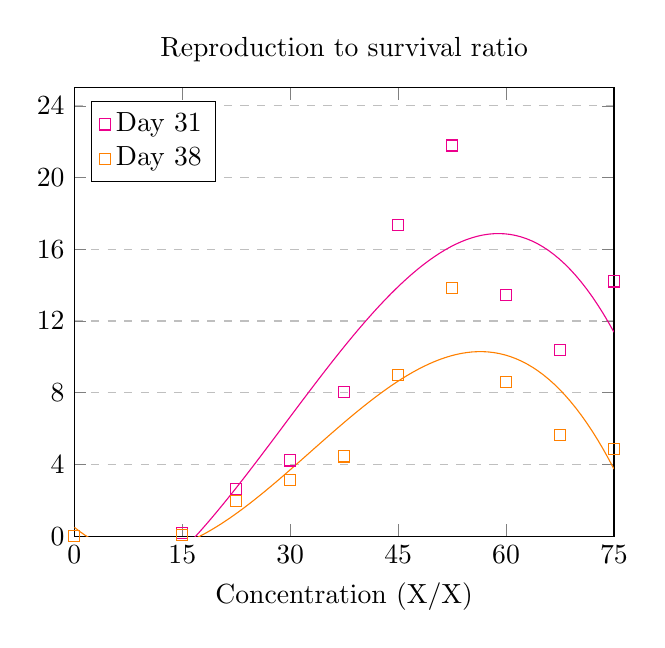
\begin{tikzpicture}
    \begin{axis}[
      title={Reproduction to survival ratio},
      xlabel={Concentration (X/X)},
      xmin=0, xmax=75,
      ymin=0, ymax=25,
      xtick={0,15,30,45,60,75},
      ytick={0,4,8,12,16,20,24},
      legend pos=north west,
      ymajorgrids=true,
      grid style=dashed,
  ]
  
    \addplot[
      only marks,
      color=magenta,
      mark=square,
    ]
    coordinates {
      (0,0)(15,0.2)(22.5,2.6316)(30,4.225)(37.5,8.0278)(45,17.3747)(52.5,21.7872)(60,13.4571)(67.5,10.3725)(75,14.2045)
    };
    \addlegendentry{Day 31}
  
    \addplot[
      only marks,
      color=orange,
      mark=square,
    ]
    coordinates {
      (0,0)(15,0.0476)(22.5,1.9608)(30,3.1296)(37.5,4.4462)(45,9.0013)(52.5,13.8378)(60,8.5813)(67.5,5.6277)(75,4.8828)
    };
    \addlegendentry{Day 38}
  
    \addplot [
      domain=0:75, 
      samples=100, 
      color=magenta,
      ]
      {-0.000203*x^3+0.01782*x^2+0.015*x-4.348499};
    \addplot [
      domain=0:75, 
      samples=100, 
      color=orange,
      ]
      {-0.000212*x^3+0.020846*x^2-0.327646*x+0.496231};
    \end{axis}
  \end{tikzpicture}
\end{minipage}
\hfill
\begin{minipage}{.45\linewidth}
  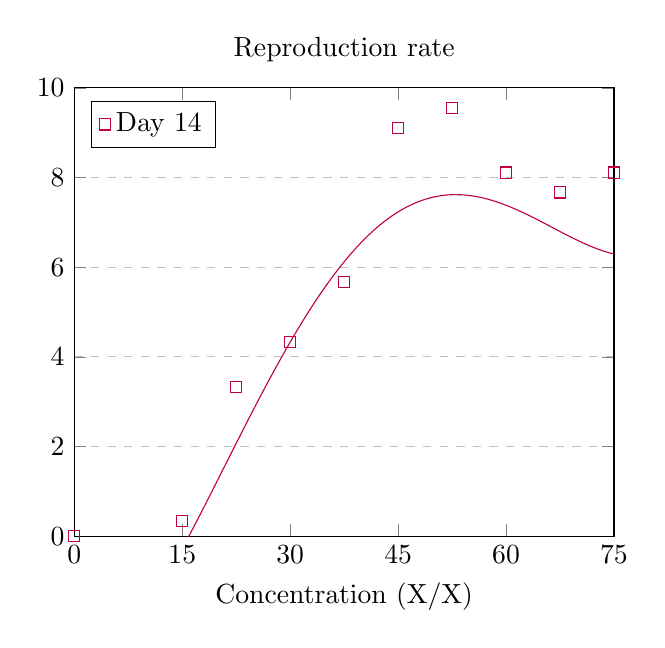
\begin{tikzpicture}
    \begin{axis}[
      title={Reproduction rate},
      xlabel={Concentration (X/X)},
      % ylabel={Reproduction rate},
      xmin=0, xmax=75,
      ymin=0, ymax=10,
      xtick={0,15,30,45,60,75},
      % ytick={0,20,40,60,80,100},
      legend pos=north west,
      ymajorgrids=true,
      grid style=dashed,
  ]
  
    \addplot[
      only marks,
      color=purple,
      mark=square,
    ]
    coordinates {
      (0,0)(15,0.3333)(22.5,3.3333)(30,4.3333)(37.5,5.6667)(45,9.1111)(52.5, 9.5556)(60, 8.1111)(67.5, 7.6667)(75, 8.1111)
    };
    \addlegendentry{Day 14}
  
    \addplot [
      domain=0:75, 
      samples=100, 
      color=purple,
      ]
      {0.0000021224*x^4-0.0003705187*x^3+0.0176288359*x^2-0.0101935078*x-2.9449417083};
    \end{axis}
  \end{tikzpicture}
\end{minipage}
\end{center}

\noindent
The graph shows that as the concentration of nutrients decreases from 45 to 0, the reproduction-to-survival ratio also drops correspondingly. This shows that at low concentrations, the reproduction rate is dropping disproportionally quicker than the survival rate, which does not support the hypothesis that fruit flies would prioritise reproduction when there are insufficient nutrients as an evolutionary feature. Instead, survival seemed to be the priority instead of reproduction when there were not enough nutrients.

\noindent\\
Not prioritising reproduction in such environments does put the drosophilas at a disadvantage when competing with a species that does this - the competitor species will explode in population size as the drosophilas decrease in population size in response, and continues to do so as the large population of the competitor species keep exhausting available food sources, leading to eventual extinction.

\noindent\\
However, there is a risk of prioritising reproduction in such environments - a minor shortage of food can lead to an increase in population, which itself leads to a more serious shortage. This chain reaction of surging population can be easily kickstarted, but difficult to end unless there is also an unlikely corresponding surge in food resources. Leaving a large, hungry population who wouldn't stop reproducing.

\noindent\\
As a result, drosophilas, and \emph{possibly all other species} would have the same behaviour of prioritising survival over reproduction when there are insufficiencies of nutrients. Assuming all species have the same behaviour, not only will they not be at a disadvantage to each other, but their population sizes will also naturally decrease and stabilise so that there is enough food for the population.

% \subsubsection{Reproduction lower threshold}
% One interesting thing to notice is that there seemed to be a threshold at around 15g/dm$^3$, where the reproduction rate would be 0 for any concentration lower than that.

% \noindent\\
% The behaviour of prioritising survival can be more simply described as so: the first 15g/dm$^3$ of culture media provides nutrients for survival purposes, any excess will then be used for reproduction. This explanation is supported by experimental data:

% \noindent\\
% In the interval of 15 to 45g/dm$^3$, the line of best fit for reproduction rate is essentially a straight line. Assuming each fly egg laid requires the same amount of energy, we can see that all (or a fixed portion of) "excess" energy is used for reproduction.

\subsection{Evalutating hypothesis: protein and carbohydrates have different functions}

The hypothesis believes that protein is specific to reproduction (and growth) while carbohydrates are specific to the flies' survival.

\noindent\\
To support this hypothesis, the experiment will need to show that when changing only the concentration of yeast or sucrose, the concentration of yeast is close to directly proportional to the reproduction rate, while the concentration of sucrose is close to directly proportional to the survival rate

\begin{center}
  
  \begin{minipage}{.45\linewidth}
    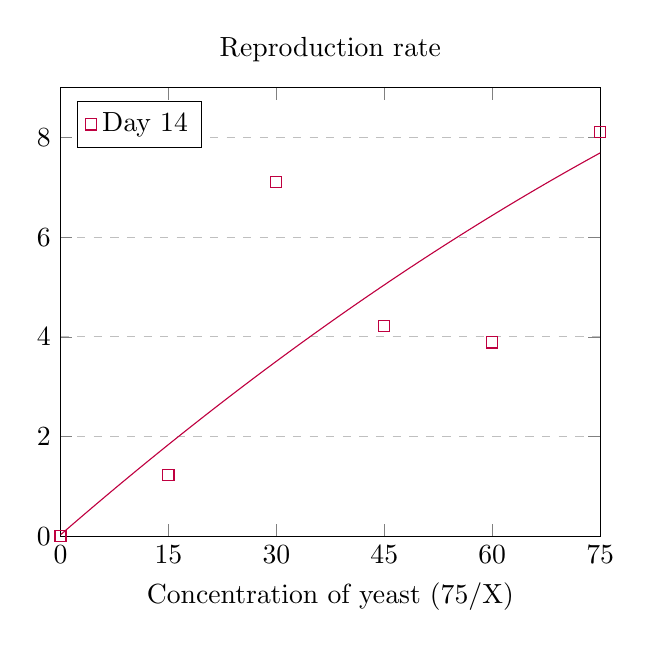
\begin{tikzpicture}
      \begin{axis}[
        title={Reproduction rate},
        xlabel={Concentration of yeast (75/X)},
        % ylabel={Reproduction divided by survival rate},
        xmin=0, xmax=75,
        ymin=0, ymax=9,
        xtick={0,15,30,45,60,75},
        ytick={0,2,4,6,8},
        legend pos=north west,
        ymajorgrids=true,
        grid style=dashed,
    ]
    
      \addplot[
        only marks,
        color=purple,
        mark=square,
      ]
      coordinates {
        (0,0)(15,1.2222)(30,7.1111)(45,4.2222)(60,3.8888)(75,8.1111)
      };
      \addlegendentry{Day 14}
    
      \addplot [
        domain=0:75, 
        samples=100, 
        color=purple,
        ]
        {-0.000308627*x^2+0.1253687381*x+0.0277821429};
      \end{axis}
    \end{tikzpicture}
    \end{minipage}
  \hfill
  \begin{minipage}{.45\linewidth}
    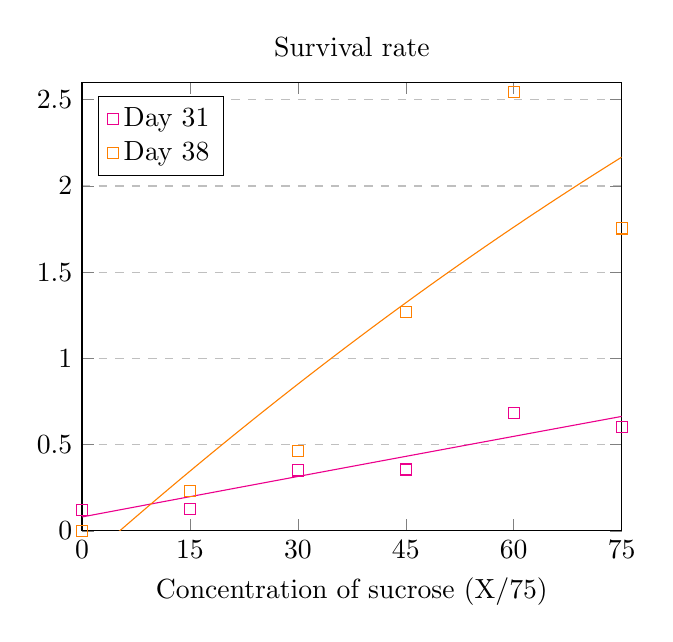
\begin{tikzpicture}
      \begin{axis}[
        title={Survival rate},
        xlabel={Concentration of sucrose (X/75)},
        % ylabel={Reproduction divided by survival rate},
        xmin=0, xmax=75,
        ymin=0, ymax=2.6,
        xtick={0,15,30,45,60,75},
        ytick={0,0.5,1,1.5,2,2.5},
        legend pos=north west,
        ymajorgrids=true,
        grid style=dashed,
    ]
    
      \addplot[
        only marks,
        color=magenta,
        mark=square,
      ]
      coordinates {
        (0,0.1204)(15,0.1264)(30,0.35)(45,0.3556)(60,0.6812)(75,0.6027)
      };
      \addlegendentry{Day 31}
    
      \addplot[
        only marks,
        color=orange,
        mark=square,
      ]
      coordinates {
        (0,0)(15,0.2299)(30,0.4625)(45,1.2667)(60,2.5429)(75,1.7534)
      };
      \addlegendentry{Day 38}
    
      \addplot [
        domain=0:75, 
        samples=100, 
        color=magenta,
        ]
        {-0.0000011508*x^2+0.0078605952*x+0.0803178571};
      \addplot [
        domain=0:75, 
        samples=100, 
        color=orange,
        ]
        {-0.0000732222*x^2+0.0369396667*x-0.19165};
      \end{axis}
    \end{tikzpicture}
    \end{minipage}
\end{center}

\noindent
(Lines of best fit are computer generated, I didn't make them up.)

\noindent\\
Although some of the individual points are far from the lines of best fit, there is a strong positive correlation between yeast and reproduction, sucrose and survival rate - they are likely directly proportional to each other. For example, doubling the amount of sucrose should double the survival rate, but not the reproduction rate. This could suggest a fixed proportion of sucrose, possibly all sucrose consumed by the flies are used to improve survival rate and nothing else. The opposite is true for yeast.

\noindent\\
It is also important to notice that vial 20 with no yeast sees the original batch of flies surviving past day 14 without any reproduction, in contrast, vial 15 the original flies only lived past day 7 but reproduced more than a hundred larvae and pupa. These larvae are not supposed to survive until the adult stage as there is no sucrose - required for survival according to the hypothesis. However, on the day 31 recording, there are indeed adult flies from the 2nd generation.

\noindent\\
After slight research, it turns out that protein offers a similar energy value as carbohydrates (their energies are both 17kJ/g)\cite{protein_energy}. This raises 2 questions:

\begin{enumerate}
  \item Concentration of yeast is directly proportional to reproduction rate, showing (likely) all protein is used for reproduction, not survival. If protein has the same energy value as carbohydrates, why isn't at least some of it used to provide energy?
  \item Why does a lower amount of sucrose lead to a lower survival rate when it can be replaced by protein?
\end{enumerate}

\noindent
(1) could be explained by \emph{hypothesising} (not tested) that drosophilas would prefer using protein for reproduction purposes when there are sufficient carbohydrates, as protein \emph{can} have the same function as carbohydrates, so with 75g/dm$^3$ of sucrose, all protein from yeast would be used in reproduction, resulting in concentration of yeast being directly proportional to reproduction rate.

\noindent\\
(2) brewers yeast consists of 44\% protein\cite{yeast_comp}, and for the same weight of sucrose and yeast, the yeast is only around half as effective as the sucrose. But this still doesn't explain why vial 9 providing an equivalent energy of only 22.5g/dm$^3$ sucrose can allow the original batch of flies to survive, while vial 15 with 35g/dm$^3$ equivalent cannot.

\noindent\\
Although not the preferred source of energy, as it cannot be stored, "proteins can also be catabolized to yield energy"\cite{protein_digestion}, so it is not clear as to why they seemingly didn't digest protein for energy when there isn't any sucrose.

\subsection{Challenges}

\subsubsection{Flies escaping}

Instead of sorting the files by gender straight into the vials, initially, I tried to do it more systematically by first separating the flies into 2 Petri dishes, one dish for males and one for females. And have the Petri dishes floating on iced water to keep the flies chill and unconscious.

\noindent\\
First of all, that is not enough to keep the flies asleep. Soon after leaving the FlyNap-filled stock vial onto the Petri dishes, they wake and start moving around. Many flew away and some climbed over the walls and jumped into the ice-cold water. Another issue with keeping flies asleep using iced water is that water condenses onto the dry side of the dish, resulting in the flies' bodies softening and clumping together like a ball of wet smudge. As well as being difficult to separate, some flies may not have survived (e.g. detaching wings) when I tried to separate them, affecting experiment results.

\noindent\\
I ended up sorting them straight to the vials, it is a quicker process and see fewer flies escaping.

\subsubsection{Limited recordings}

There were only 5 recordings in this investigation, and mostly only recordings on day 31 and day 38 can be used for evaluating results. In occasions where trends shown in the two recordings do not align with each other, I have no third recording to reference.

\noindent\\
There are not enough recordings for testing the \emph{protein/carbohydrates specific functions}. Although the lines of best fit support the hypothesis, the trend is not obvious with only 6 points, and more vials for that could make the trend more obvious.

\newpage
\noindent
A better investigation would include larger vials so the investigation can have a longer duration with more recordings. Also, more vials so that there can be more points to put on graphs, allowing trends to be identified with higher confidence.

\subsubsection{Evaluating}

This investigation report is rewritten from scratch, as the previous version is terribly structured and has an uninteresting evaluation section. The hardest part of the evaluation is to come up with different ways to visualise data, as it enables me to spot patterns I previously didn't know existed.

\noindent\\
For example, I noticed there's a positive correlation between sucrose and survival rate, but I didn't know that they are directly proportional when I first wrote the evaluation section, as I was using \emph{reproduction-to-survival ratio} to evaluate the hypothesis. Visualising the reproduction rate and survival rate allows me to see that they are indeed directly proportional.

\noindent\\
When I first made the graph of the reproduction rate, I also included point (0, 0). This made the line of best fit ease out near 0 and did not show that between 15 and 45g/dm$^3$, the relation between reproduction and concentration is linear, but when I rewrote this I realised that 0 does not need to be included. Revisiting experimental data is really useful for drawing comprehensive conclusions.

\subsection{Further investigations}

The results of this investigation raised some questions unanswered.

\begin{enumerate}
  \item 3.4 shows that the reproduction rate is directly proportional to the concentration of yeast, but as displayed in the graph on page 13, the reproduction rate does not start climbing until 15g/dm$^3$ when sucrose is at a lower amount. These two trends do not coincide with each other.
  \item Top of page 15, why do flies not use protein as a source of energy?
  \item Find a mathematical way to predict the survival/reproduction rate from the vial's composition. Currently, linear relationships between sucrose/yeast and survival/reproduction can be seen, but there are still unexplained behaviours, and more vials with different compositions are needed to map out the lines of best fit more precisely.
\end{enumerate}

\newpage
\begin{thebibliography}{unsrt}
    \bibitem{wiki_fly} \emph{Drosophila melanogaster - Lifecycle and reproduction} (Wikipedia).
    \bibitem{alzheimers} \emph{Fruit flies help researchers decode genetic link to Alzheimer's disease} (Science News, 9th Jan 2023).
    \bibitem{fly_facts} \emph{Why use the fly in research?} (yourgenome.org)
    \bibitem{sim_recipe} \emph{BDSC Cornmeal Food} (blogs.cornell.edu)
    \bibitem{diet} \emph{Experimental diets in Drosophila research} from \emph{Drosophila melanogaster in nutrition research} (Biomed Central, 1st Feb 2019)
    \bibitem{in_medium} \emph{Larval Stages} from \emph{Drosophila Development: Stages, Significance} (thebiologynotes.com)
    \bibitem{protein_energy} \emph{3.5.1 Calculation of the energy content of foods - energy conversion factors} from \emph{FAO} (www.fao.org)
    \bibitem{yeast_comp} \emph{Brewers yeast, dried} from \emph{Feedtables} (www.feedtables.com)
    \bibitem{protein_digestion} \emph{What fuels the fly: Energy metabolism in Drosophila and its application to the study of obesity and diabetes} from \emph{National Library of Medicine} (www.ncbi.nlm.nih.gov)
\end{thebibliography}

\thispagestyle{fancy}
\pagenumbering{gobble}
\fancyhead{}
\renewcommand{\headrulewidth}{0pt}
\fancyfoot[L]{Written with \LaTeX}
\fancyfoot[R]{Source availabe on siriusmart.github.io/crest2023}
\end{document}